\chapter{Appendix}
\label{apx:appendix}

\clearpage
\section{Monsoon Onset Dates}
\label{apx:onset_dates}

\begin{figure}[h]
  \centering
  \begin{tabular}{cc}
    \subfloat{
      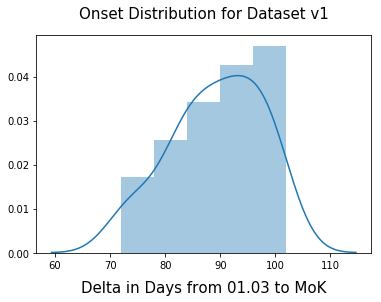
\includegraphics[width = 0.3\linewidth]{./99_appendix/img/onset_hist_v1}} &
    \subfloat{
      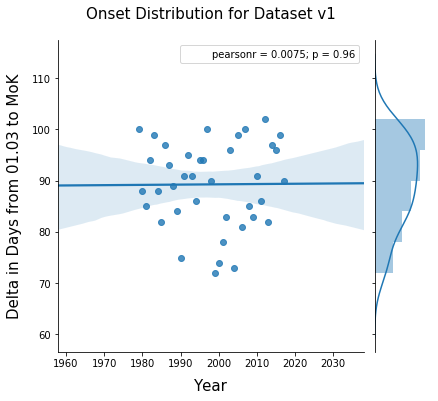
\includegraphics[width = 0.35\linewidth]{./99_appendix/img/onset_joint_v1}} \\
    \subfloat{
      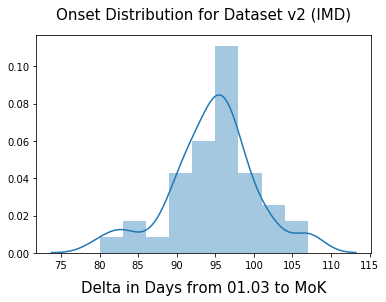
\includegraphics[width = 0.3\linewidth]{./99_appendix/img/onset_hist_v2_imd}} &
    \subfloat{
      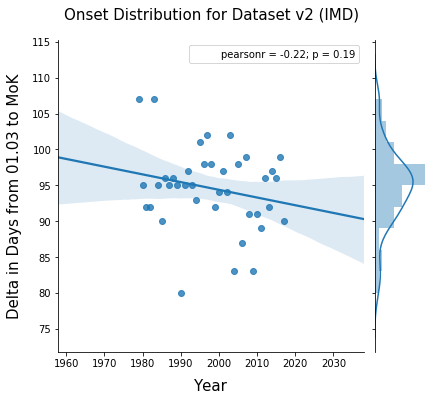
\includegraphics[width = 0.35\linewidth]{./99_appendix/img/onset_joint_v2_imd}} \\
    \subfloat{
      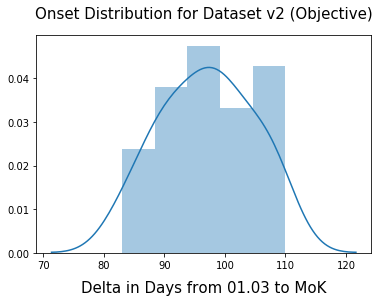
\includegraphics[width = 0.3\linewidth]{./99_appendix/img/onset_hist_v2_obj}} &
    \subfloat{
      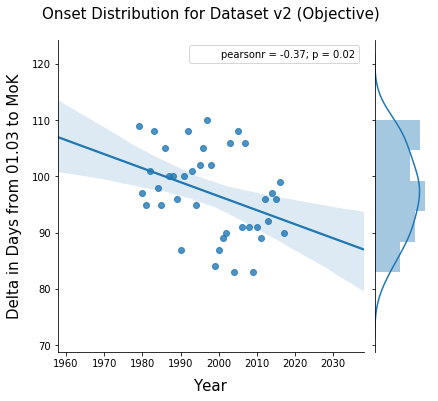
\includegraphics[width = 0.35\linewidth]{./99_appendix/img/onset_joint_v2_obj}} \\
  \end{tabular}
  \caption{Overview of Onset Distributions (1979-2017, v1: \citet{Ordonez.2016, IndiaMeteorologicalDepartment.2017b}, v2: \citet{Singh.2009, IndiaMeteorologicalDepartment.2017b}}
  \label{apx:onset_distributions}
\end{figure}

\begin{figure}[h]
  \centering
  \begin{tabular}{cc}
    \subfloat{
      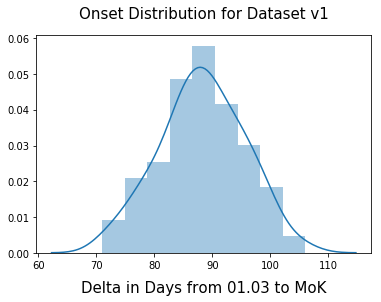
\includegraphics[width = 0.3\linewidth]{./99_appendix/img/onset_hist_v1_uncut}} &
    \subfloat{
      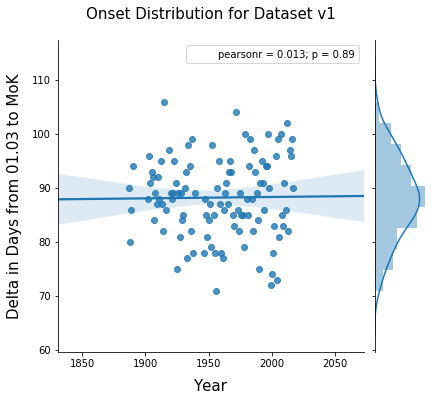
\includegraphics[width = 0.35\linewidth]{./99_appendix/img/onset_joint_v1_uncut}} \\
    \subfloat{
      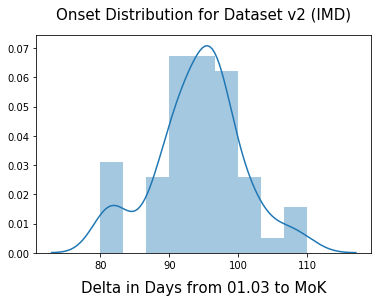
\includegraphics[width = 0.3\linewidth]{./99_appendix/img/onset_hist_v2_imd_uncut}} &
    \subfloat{
      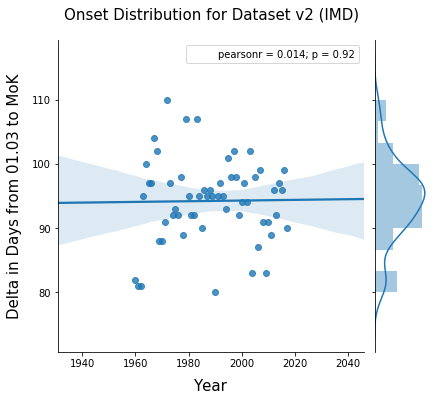
\includegraphics[width = 0.35\linewidth]{./99_appendix/img/onset_joint_v2_imd_uncut}} \\
    \subfloat{
      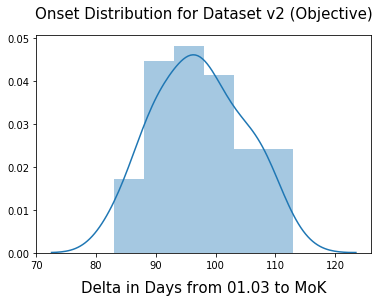
\includegraphics[width = 0.3\linewidth]{./99_appendix/img/onset_hist_v2_obj_uncut}} &
    \subfloat{
      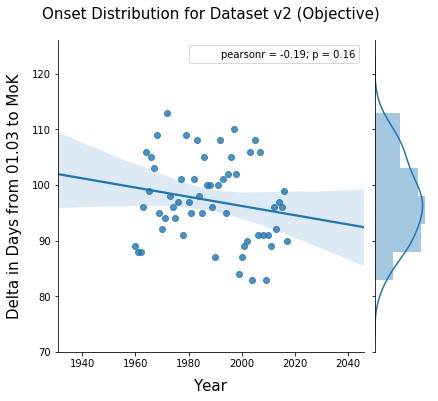
\includegraphics[width = 0.35\linewidth]{./99_appendix/img/onset_joint_v2_obj_uncut}} \\
  \end{tabular}
  \caption{Overview of Onset Distributions (v1: 1887-2017, \citet{Ordonez.2016, IndiaMeteorologicalDepartment.2017b}, v2: 1960-2017, \citet{Singh.2009, IndiaMeteorologicalDepartment.2017b})}
  \label{apx:onset_distributions_uncut}
\end{figure}

\clearpage
\section{TRMM \& ERA}
\label{apx:trmm_era}

\subsection{Getting the datasets}
\label{apx:download}
\begin{itemize}
  \item TODO: Subsetting and Downloading (with Giovanni etc.)
\end{itemize}

\subsection{Usage with Python}
\begin{itemize}
  \item TODO: NetCDF4 vs. GRIB
  \item TODO: Python Libraries for handling NetCDF4
  \item TODO: Pseudocode for import
\end{itemize}

\clearpage
\subsection{Feature analysis}
\label{apx:era_features}
The visualizations in this section show the development of different relevant ERA and TRMM features over the duration of an average monsoon. To calculate the visualizations, the data for each feature has been averaged over all years available (1998-2017 for TRMM, 1979-2017 for ERA).

\textbf{Example:} The temperature grids 10 days previous to the objective onset dates (MoK; \ref{apx:era_t}) for all available years are extracted and then averaged to yield an averaged grid representation. The visualization is then simply calculated based on the averaged grid.

\begin{figure}[h]
  \centering
  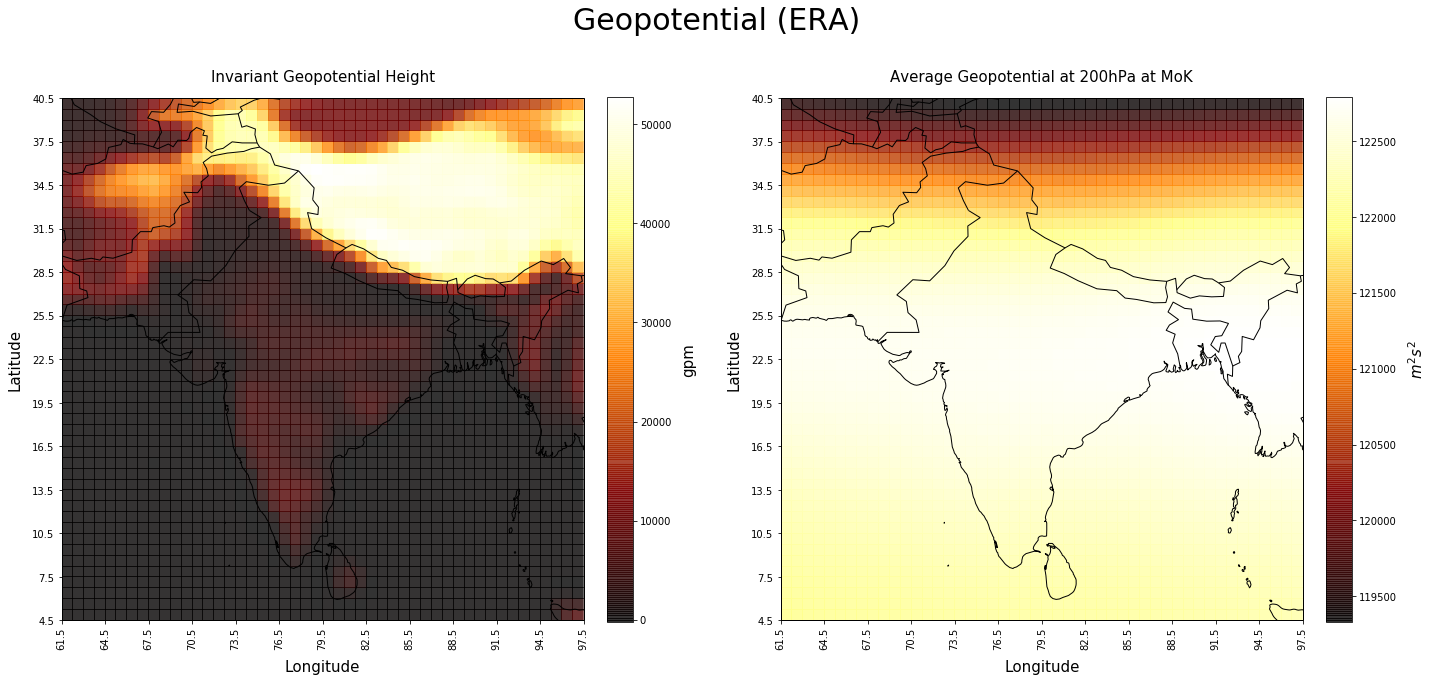
\includegraphics[width=\linewidth]{./99_appendix/img/geopotential}
  \caption{Geopotential Height and Geopotential at 200hPa (ERA-Interim, 1979-2017)}
  \label{apx:era_geopotential}
\end{figure}

\begin{figure}[h]
  \centering
  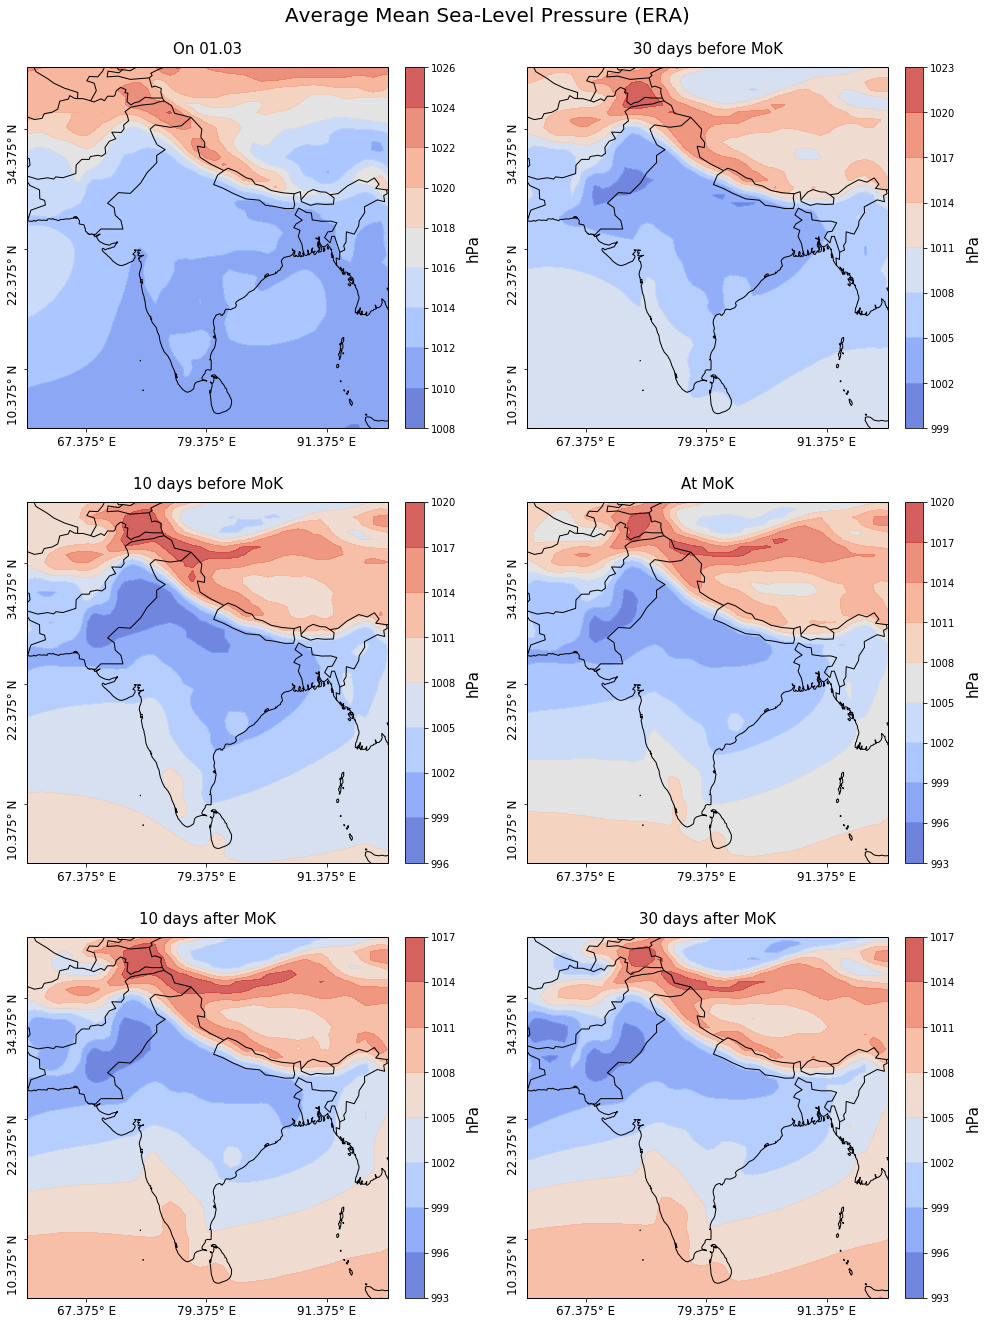
\includegraphics[width=\linewidth]{./99_appendix/img/msl_avg}
  \caption{Average Mean Sea-Level Pressure (ERA-Interim, 1979-2017)}
  \label{apx:era_msl}
\end{figure}

\begin{figure}[h]
  \centering
  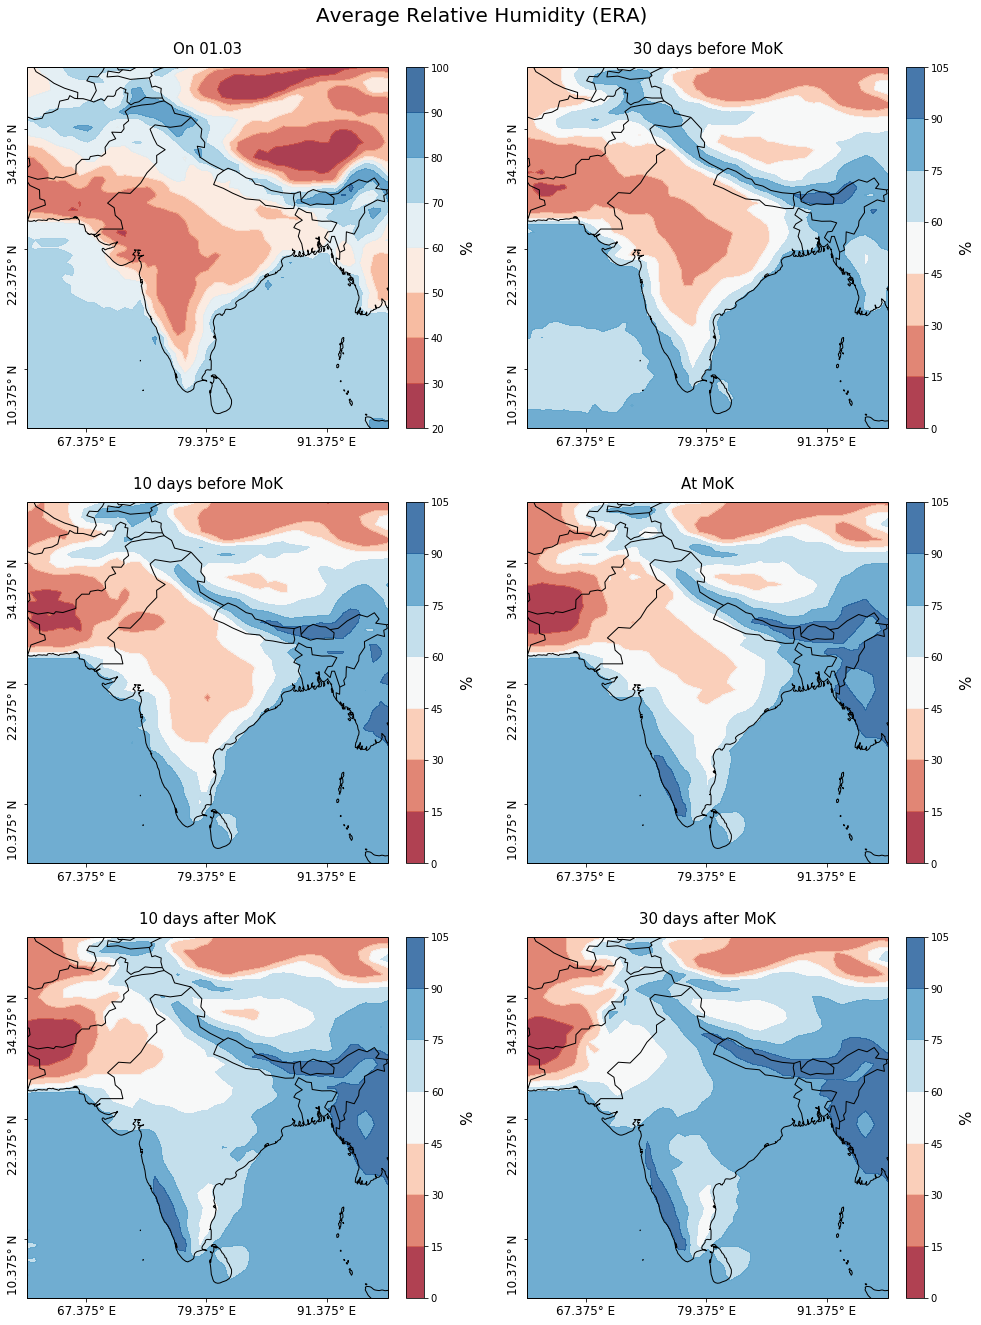
\includegraphics[width=\linewidth]{./99_appendix/img/r_avg}
  \caption{Average Relative Humidity at 1000hPa (ERA-Interim, 1979-2017)}
  \label{apx:era_r}
\end{figure}

\begin{figure}[h]
  \centering
  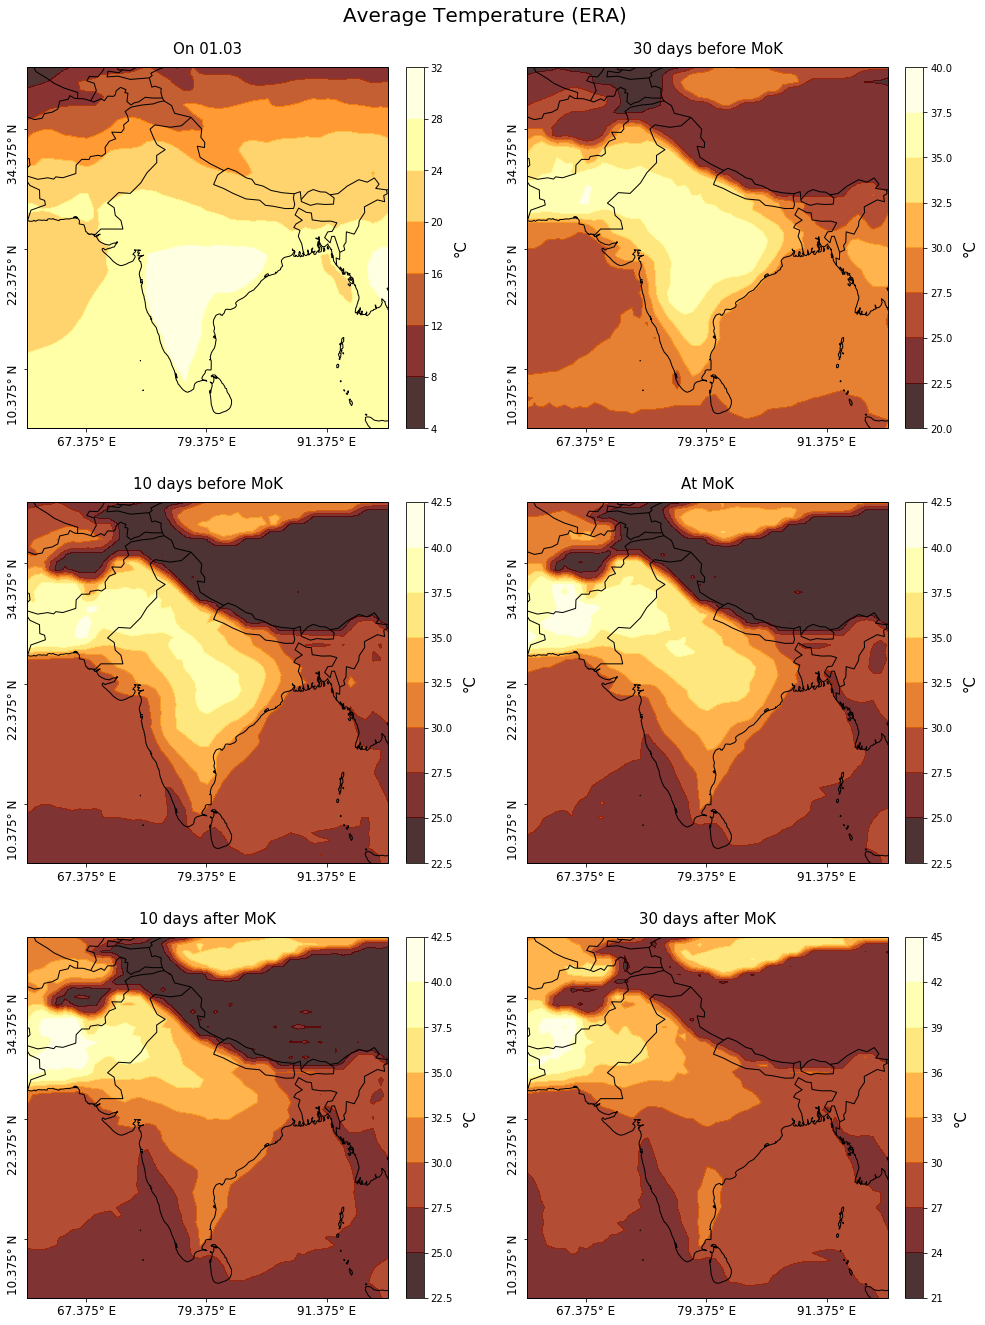
\includegraphics[width=\linewidth]{./99_appendix/img/t_avg}
  \caption{Average Temperature at 1000hPa (ERA-Interim, 1979-2017)}
  \label{apx:era_t}
\end{figure}

\begin{figure}[h]
  \centering
  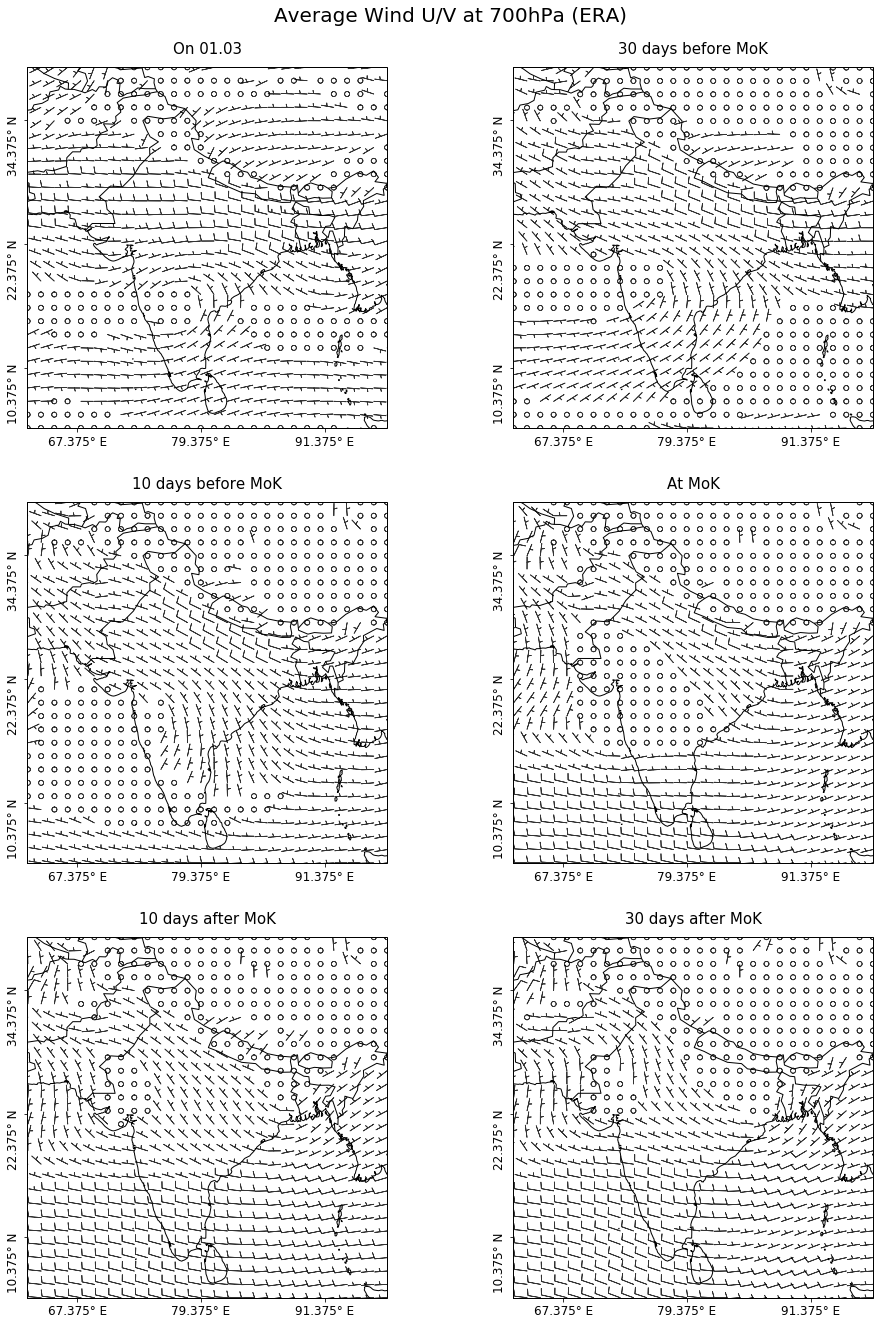
\includegraphics[width=\linewidth]{./99_appendix/img/wind_avg}
  \caption{Average Wind (U/V) at 700hPa (ERA-Interim, 1979-2017)}
  \label{apx:era_wind}
\end{figure}

\begin{figure}[h]
  \centering
  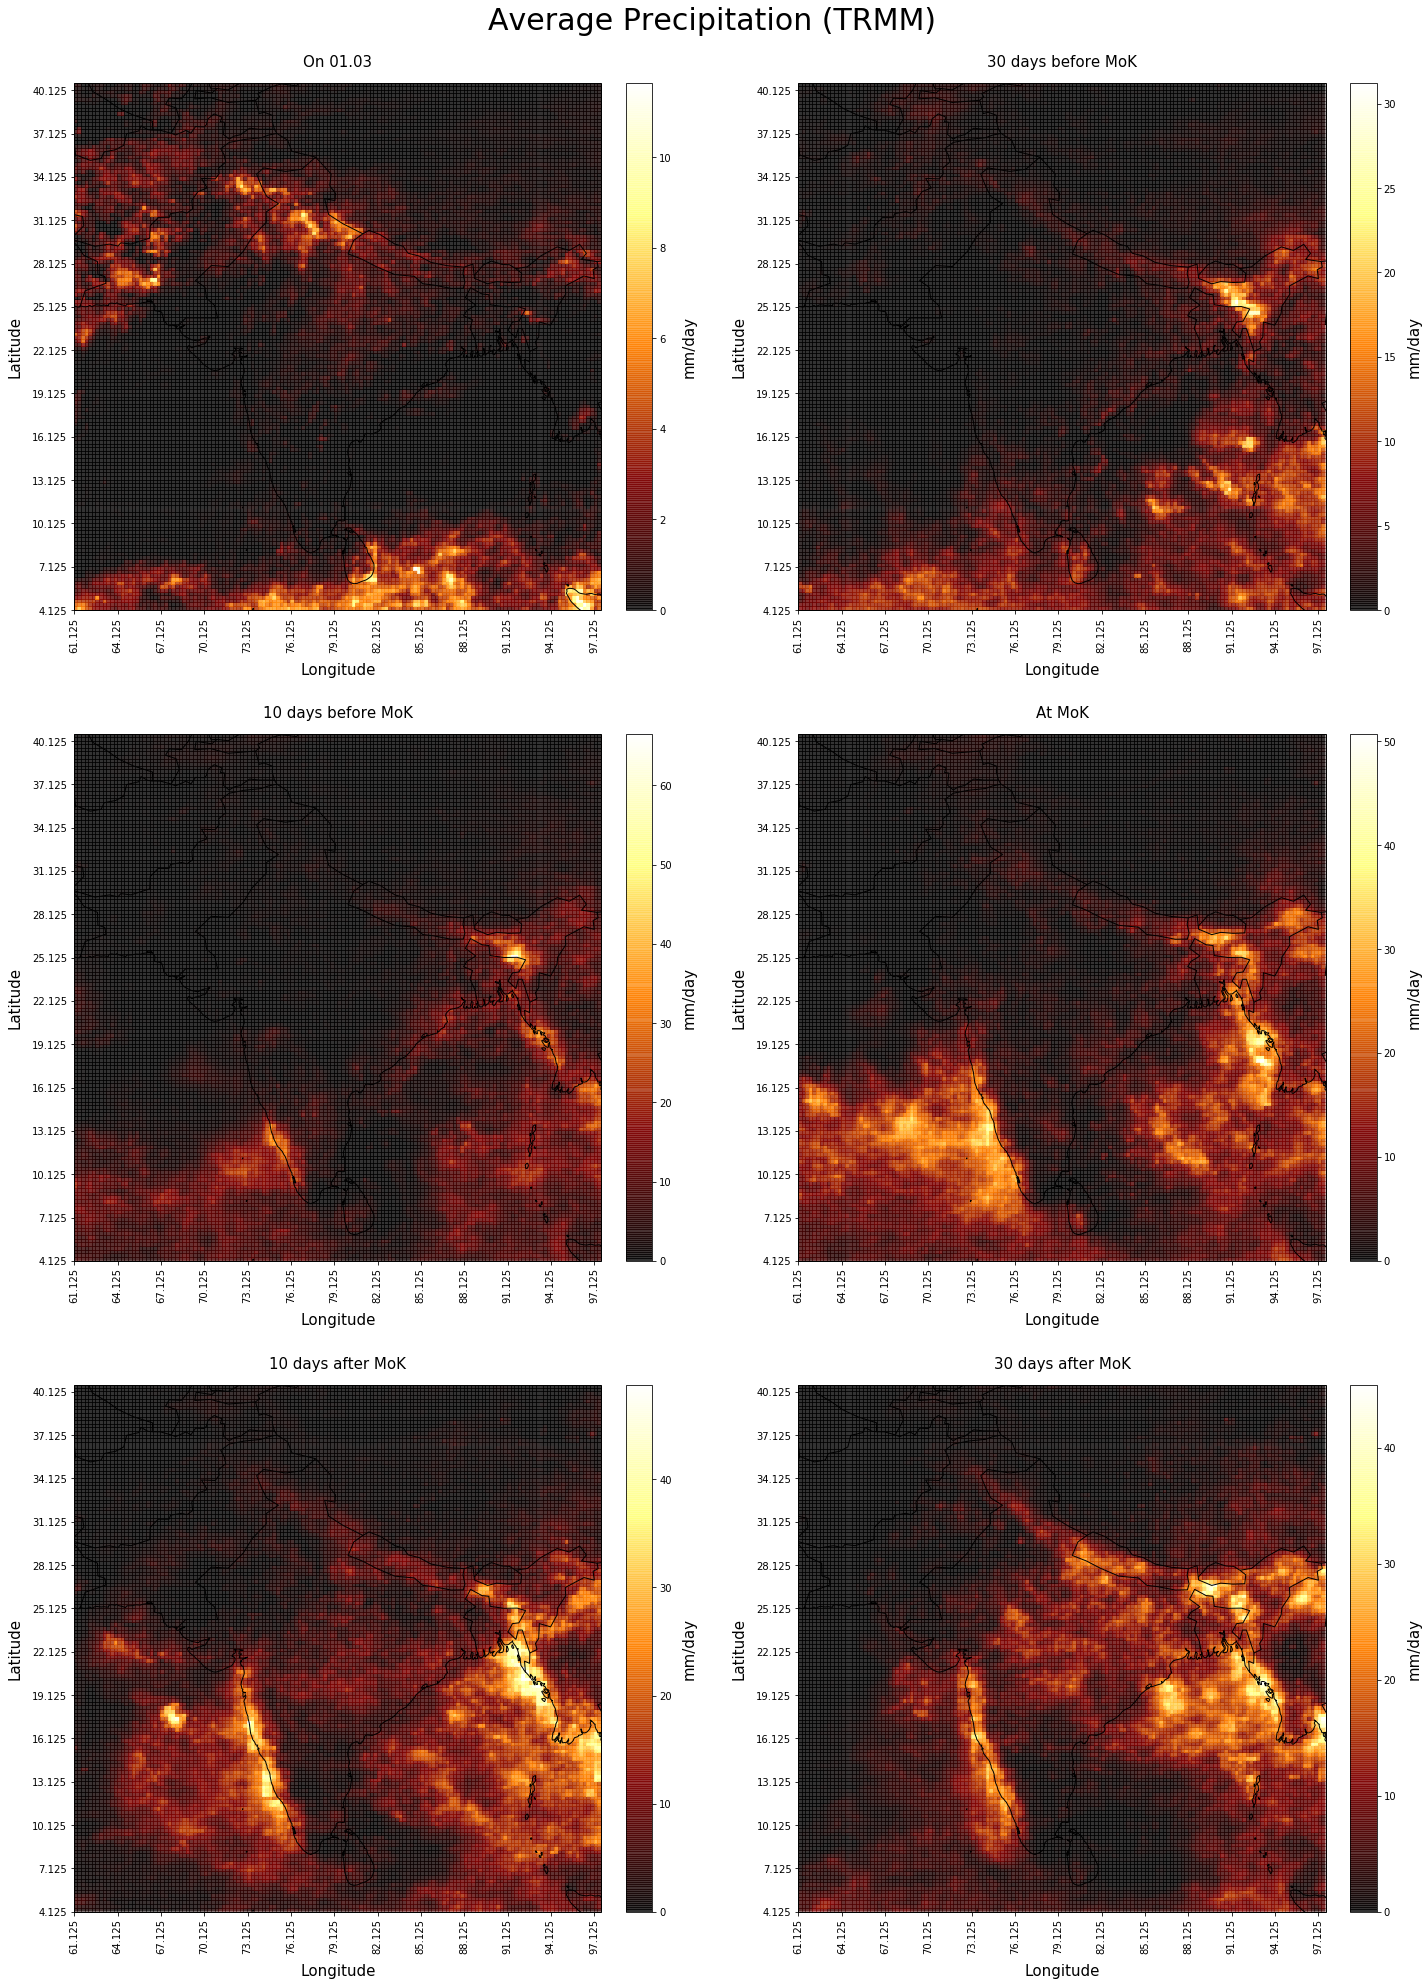
\includegraphics[width=\linewidth]{./99_appendix/img/prec_avg}
  \caption{Average Precipitation (TRMM, 1998-2017)}
  \label{apx:trmm_prec}
\end{figure}

\clearpage
\section{Event Synchronization}
\label{apx:event_sync}

\begin{figure}[h]
  \centering
  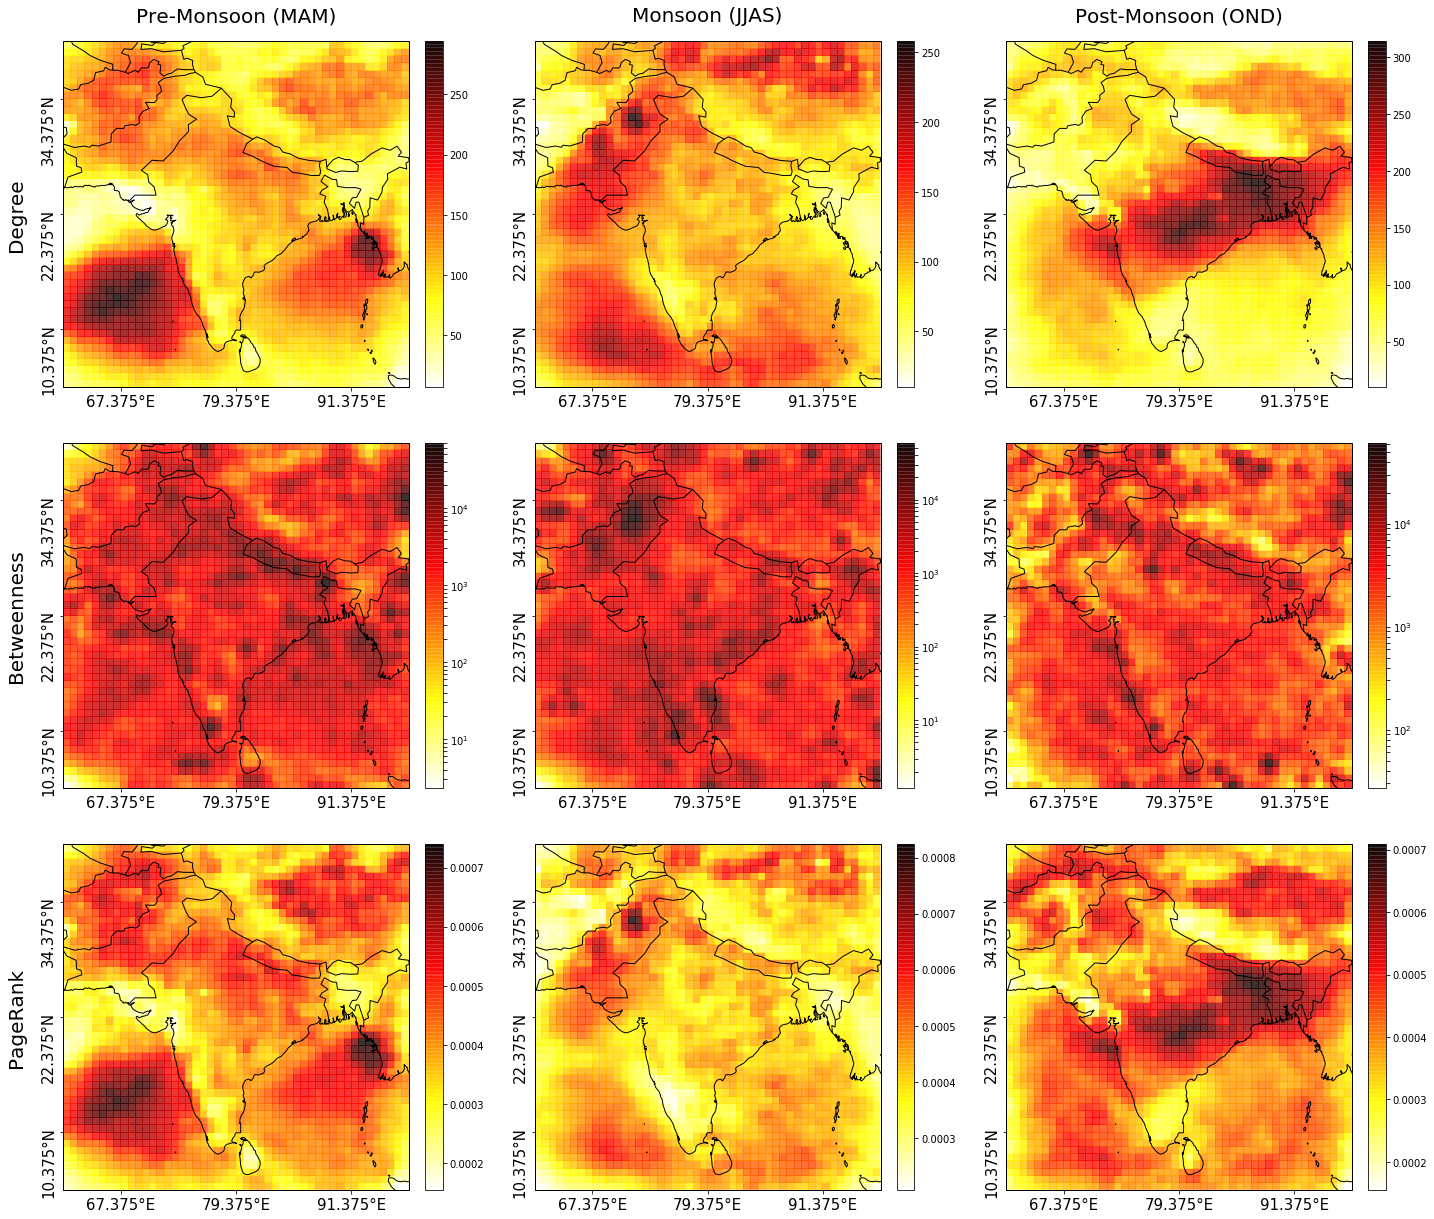
\includegraphics[width=\linewidth]{{./99_appendix/img/event_sync_0.75-0.9}.png}
  \caption{Climate network analysis for unweighted, undirected climate networks (based on TRMM at {0.75\degree} resolution and a threshold set at the 95th percentile).}
  \label{apx:climate_network_basic}
\end{figure}

\begin{figure}[h]
  \centering
  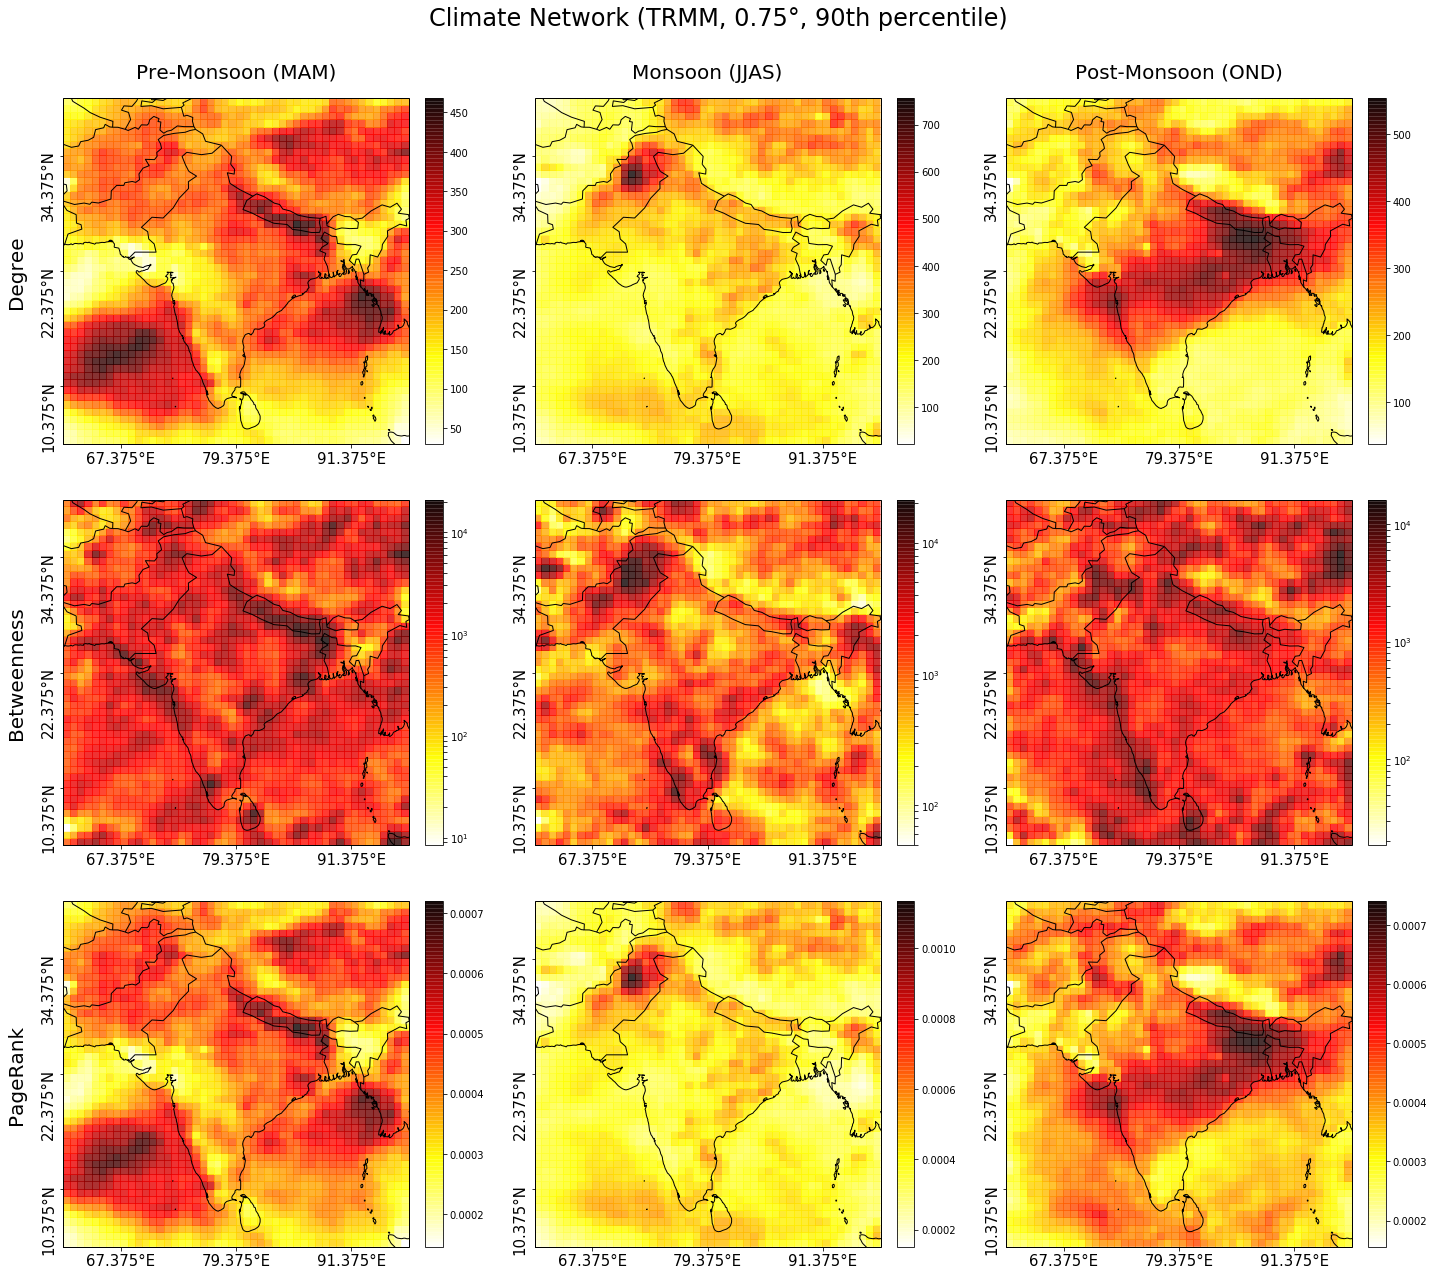
\includegraphics[width=\linewidth]{{./99_appendix/img/event_sync_0.75-0.9_90}.png}
  \caption{Climate network analysis for unweighted, undirected climate networks (based on TRMM at {0.75\degree} resolution and a threshold set at the 90th percentile).}
  \label{apx:climate_network_basic_90}
\end{figure}

\begin{figure}[h]
  \centering
  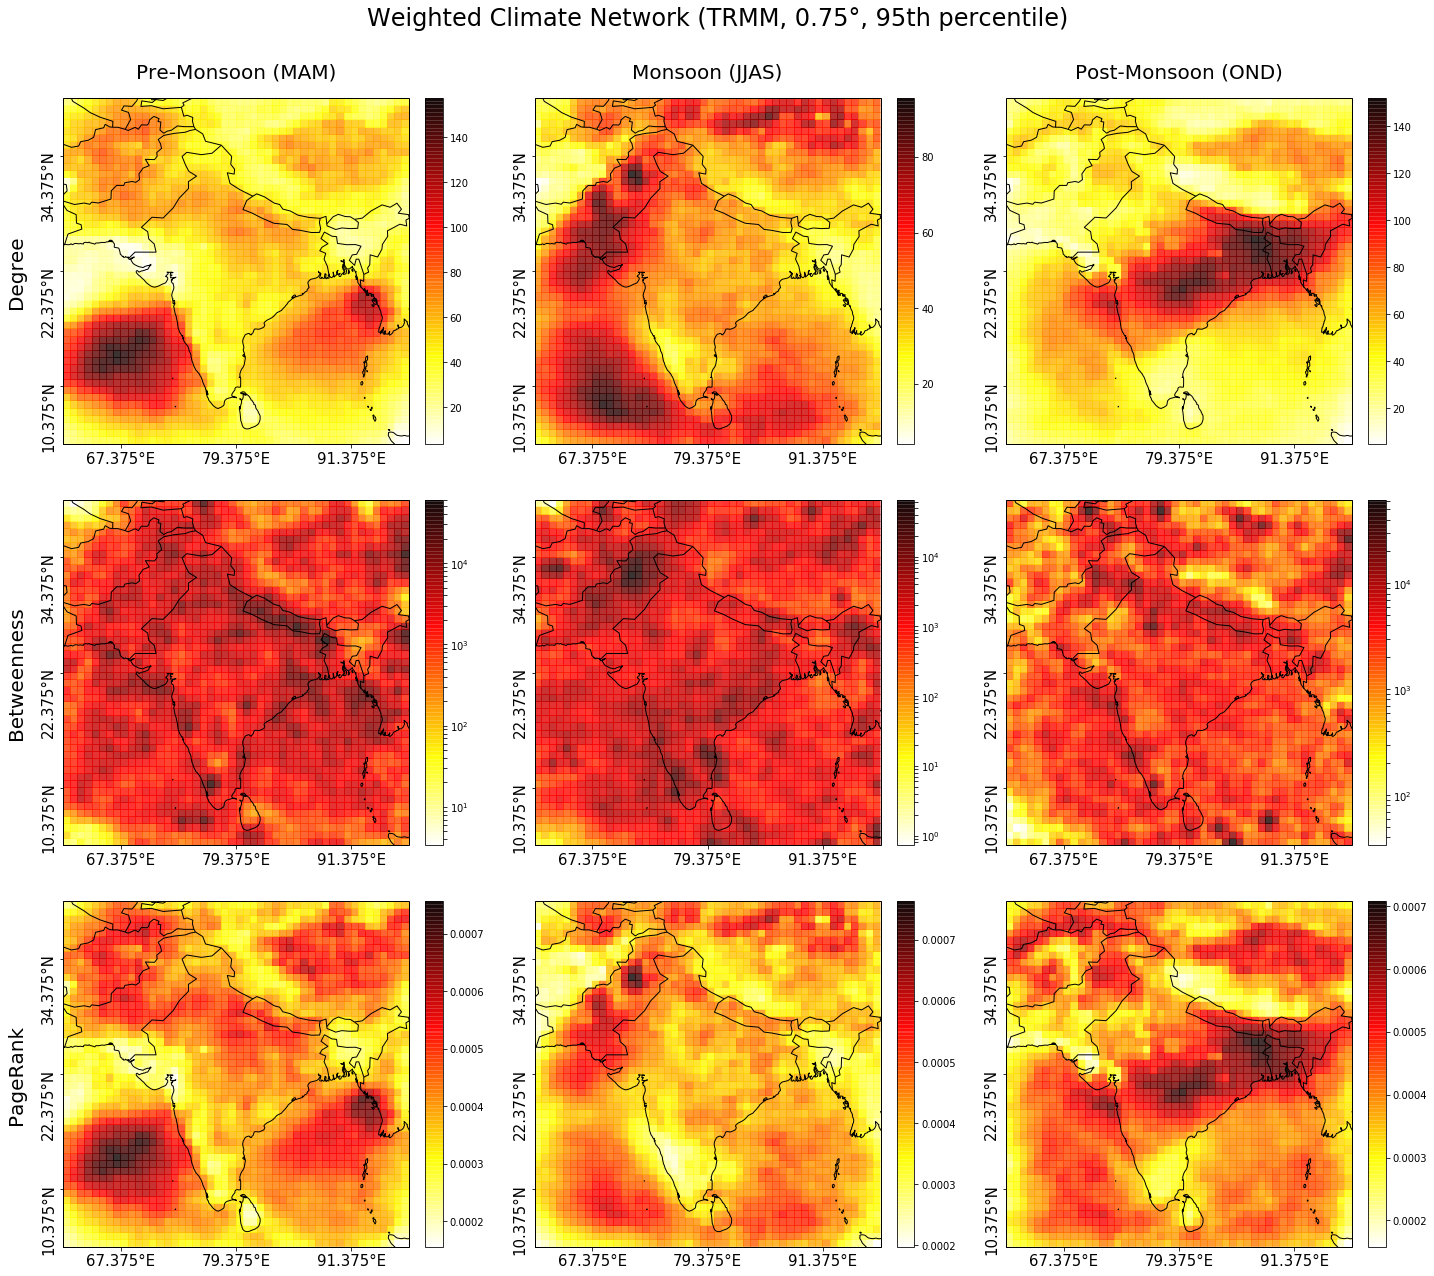
\includegraphics[width=\linewidth]{{./99_appendix/img/event_sync_0.75-0.9_weighted}.png}
  \caption{Climate network analysis for weighted, undirected climate networks (based on TRMM at {0.75\degree} resolution and a threshold set at the 95th percentile).}
  \label{apx:climate_network_weighted}
\end{figure}

\begin{figure}[h]
  \centering
  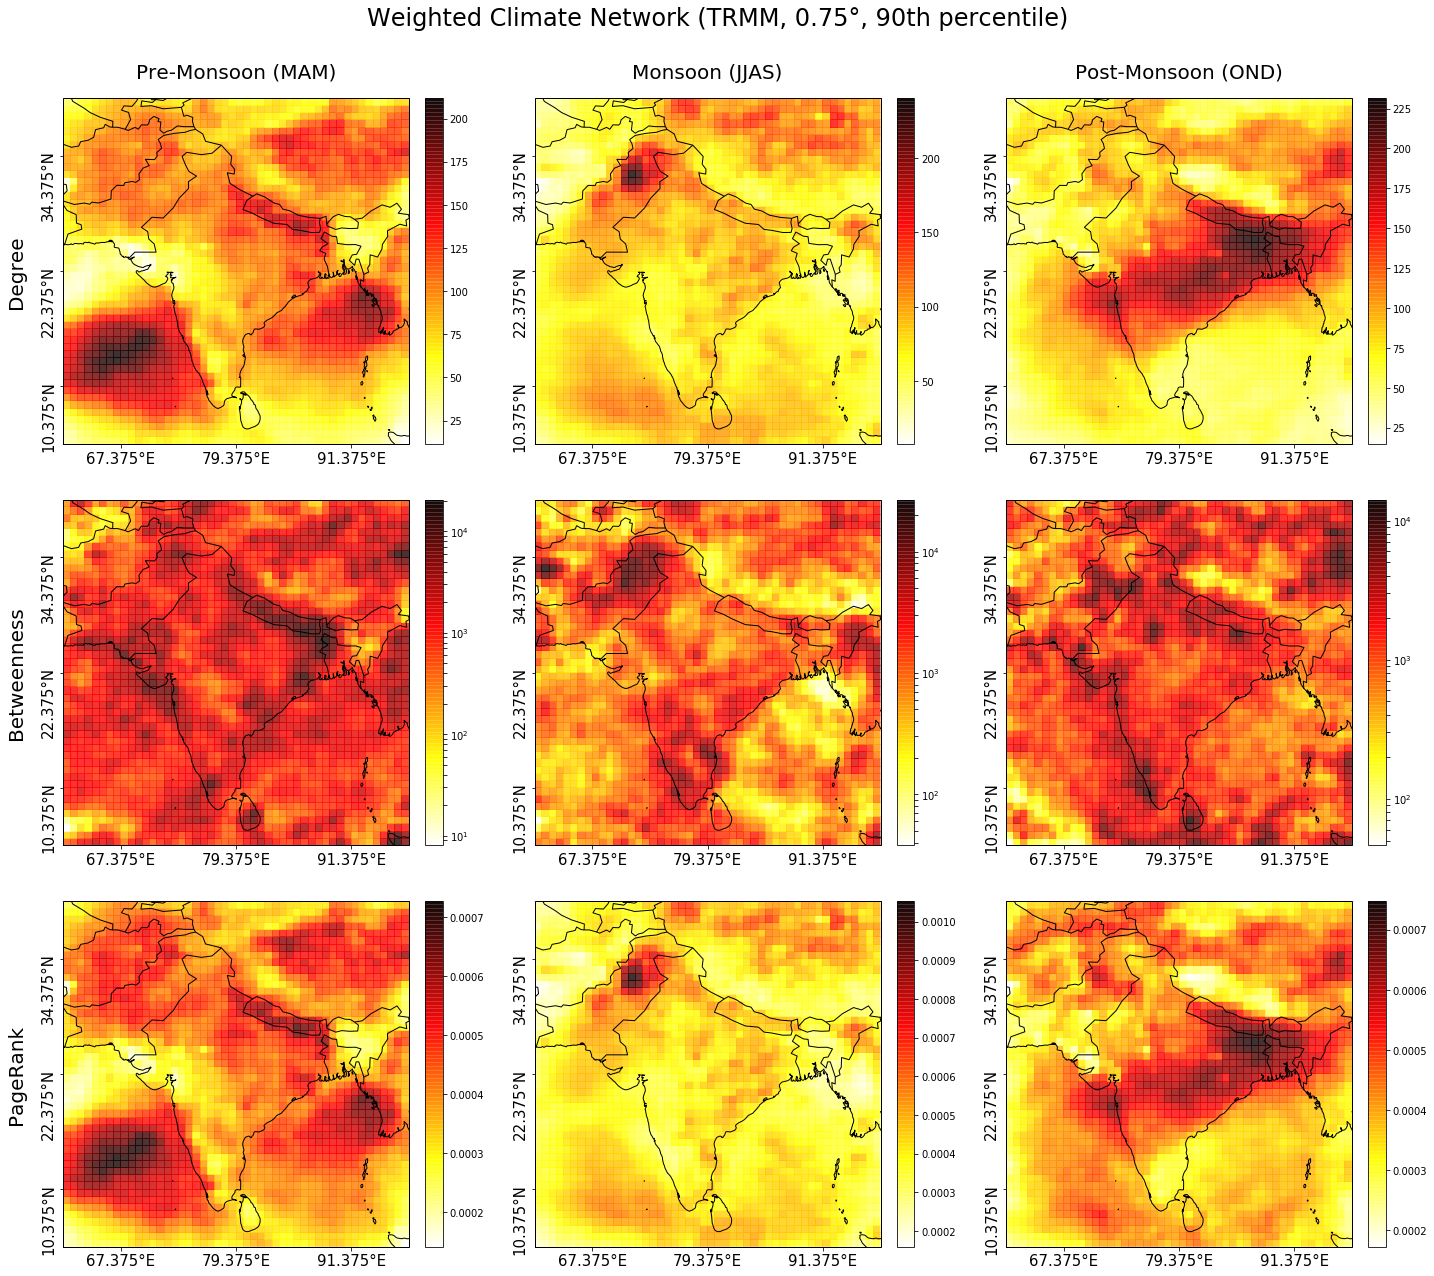
\includegraphics[width=\linewidth]{{./99_appendix/img/event_sync_0.75-0.9_weighted_90}.png}
  \caption{Climate network analysis for weighted, undirected climate networks (based on TRMM at {0.75\degree} resolution and a threshold set at the 90th percentile).}
  \label{apx:climate_network_weighted_90}
\end{figure}

\begin{figure}[h]
  \centering
  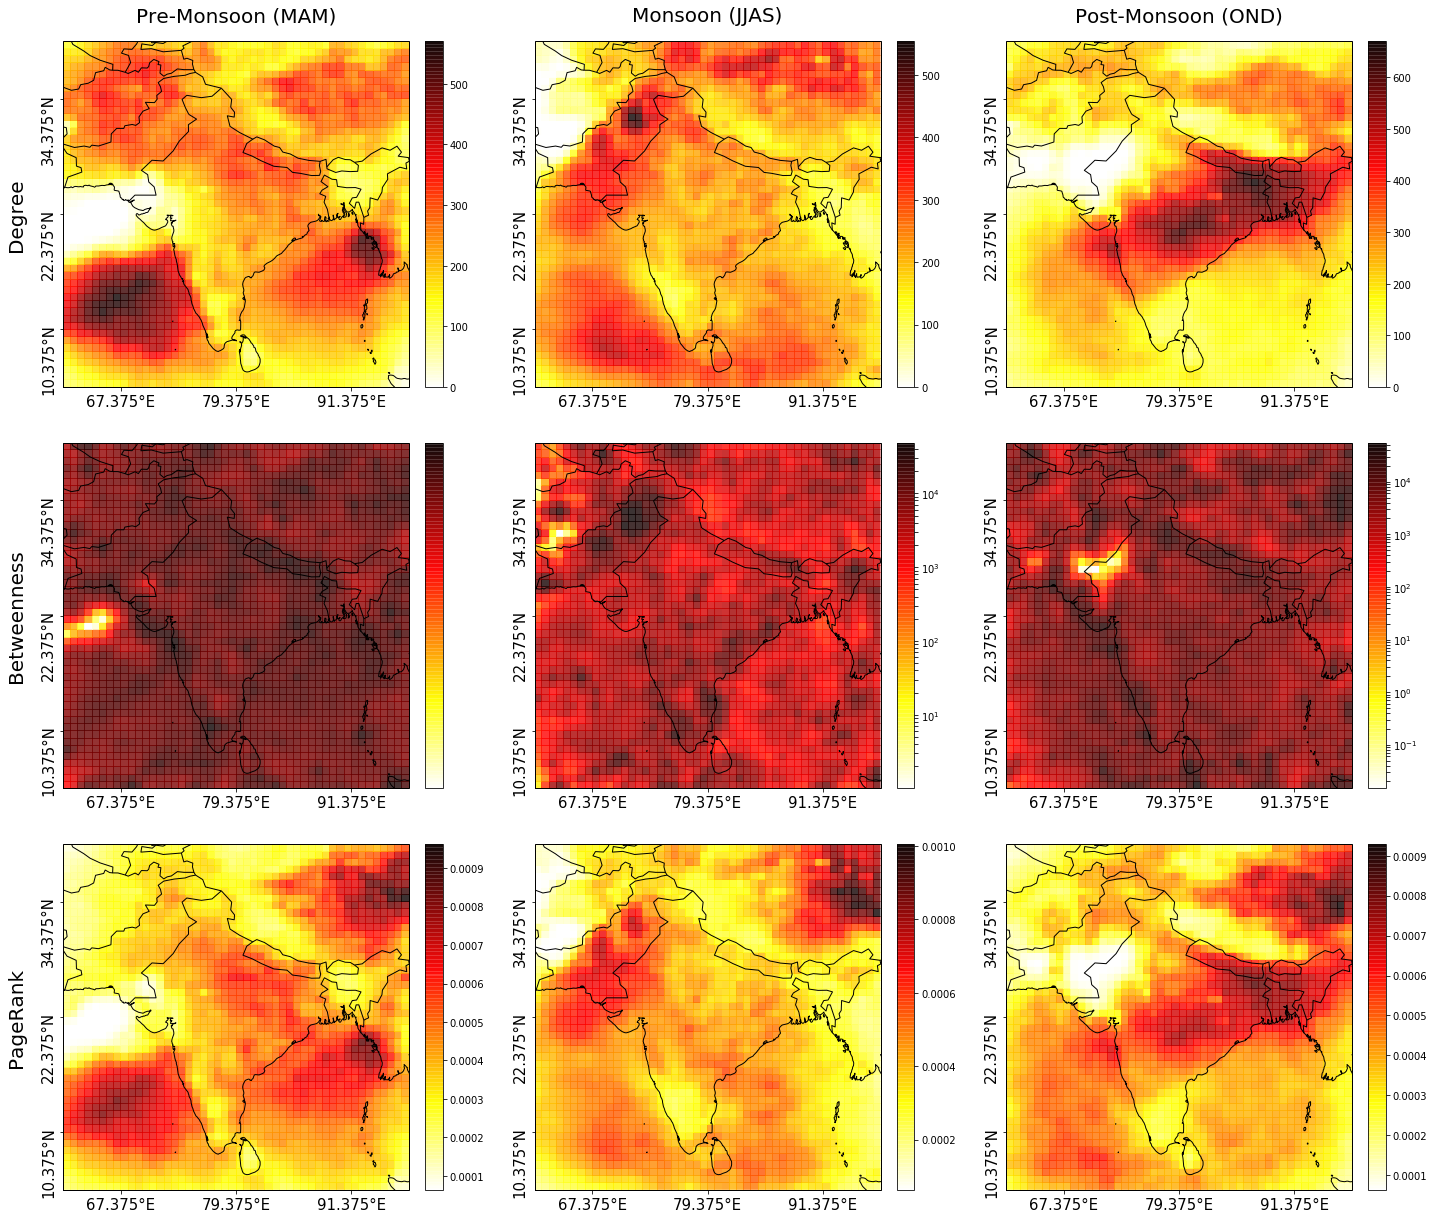
\includegraphics[width=\linewidth]{{./99_appendix/img/event_sync_0.75-0.9_directed}.png}
  \caption{Climate network analysis for unweighted, directed climate networks (based on TRMM at {0.75\degree} resolution and a threshold set at the 95th percentile).}
  \label{apx:climate_network_directed}
\end{figure}

\begin{figure}[h]
  \centering
  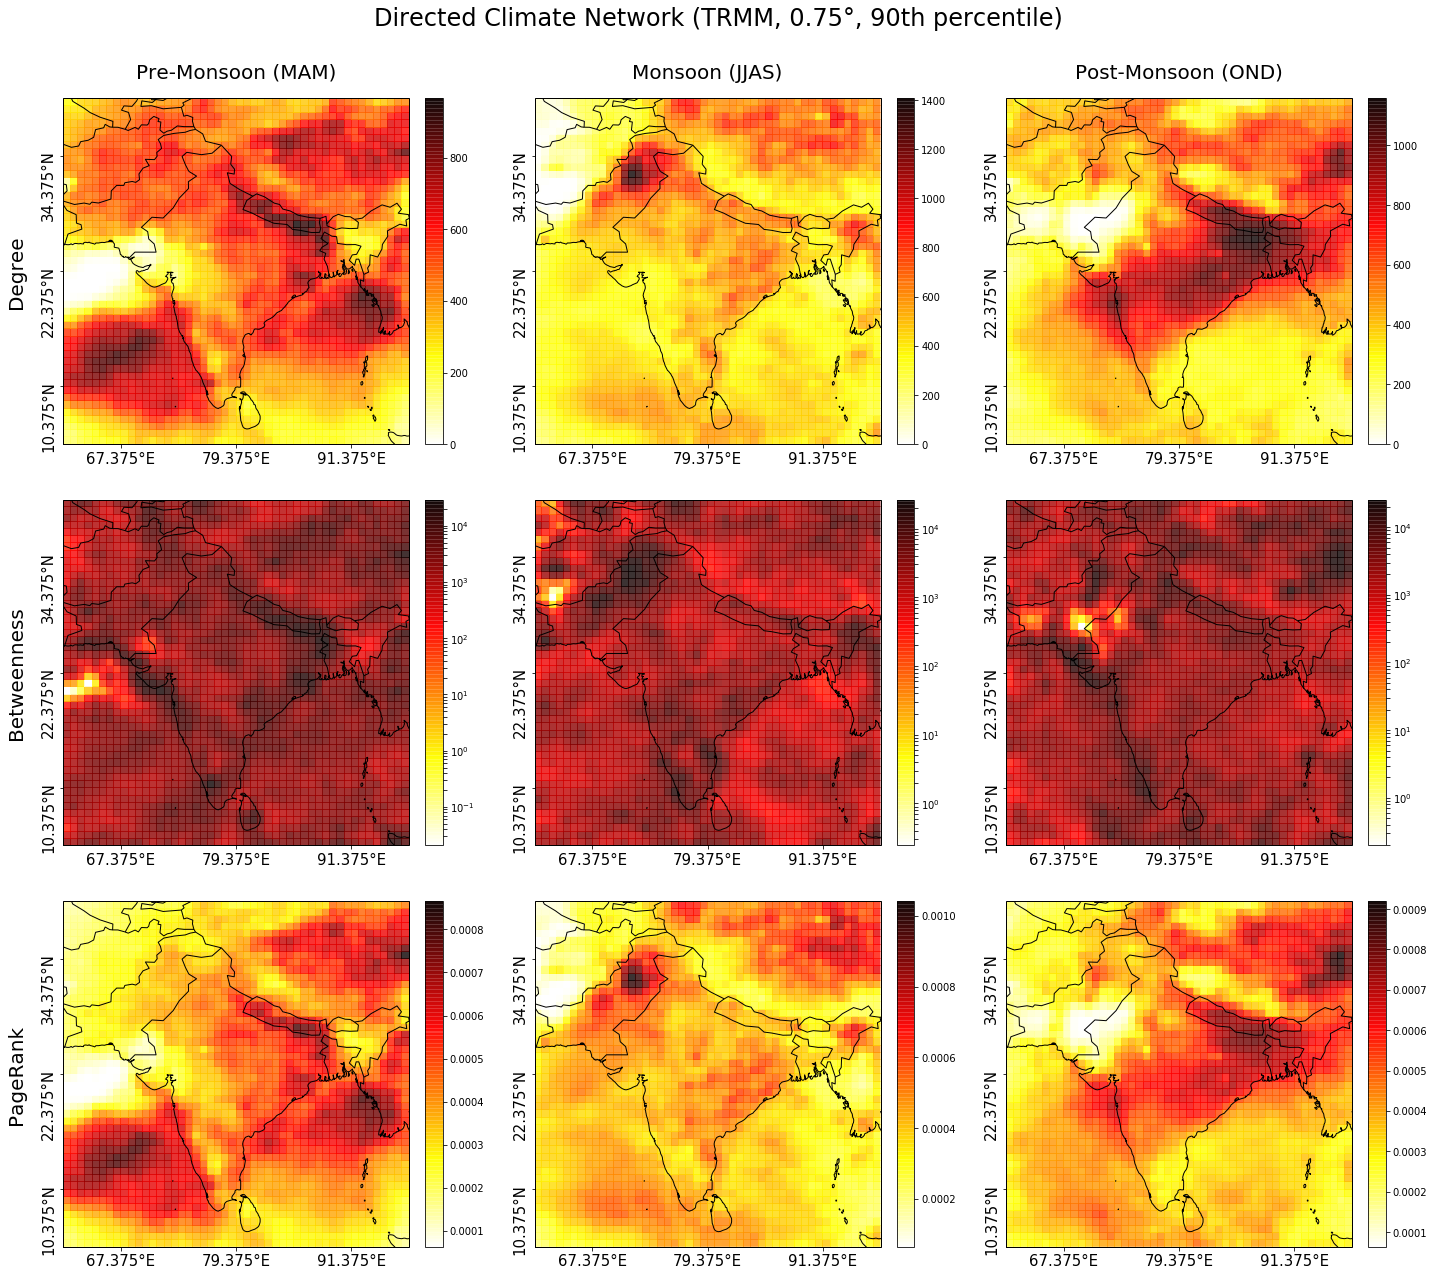
\includegraphics[width=\linewidth]{{./99_appendix/img/event_sync_0.75-0.9_directed_90}.png}
  \caption{Climate network analysis for unweighted, directed climate networks (based on TRMM at {0.75\degree} resolution and a threshold set at the 90th percentile).}
  \label{apx:climate_network_directed}
\end{figure}

\begin{figure}[h]
  \centering
  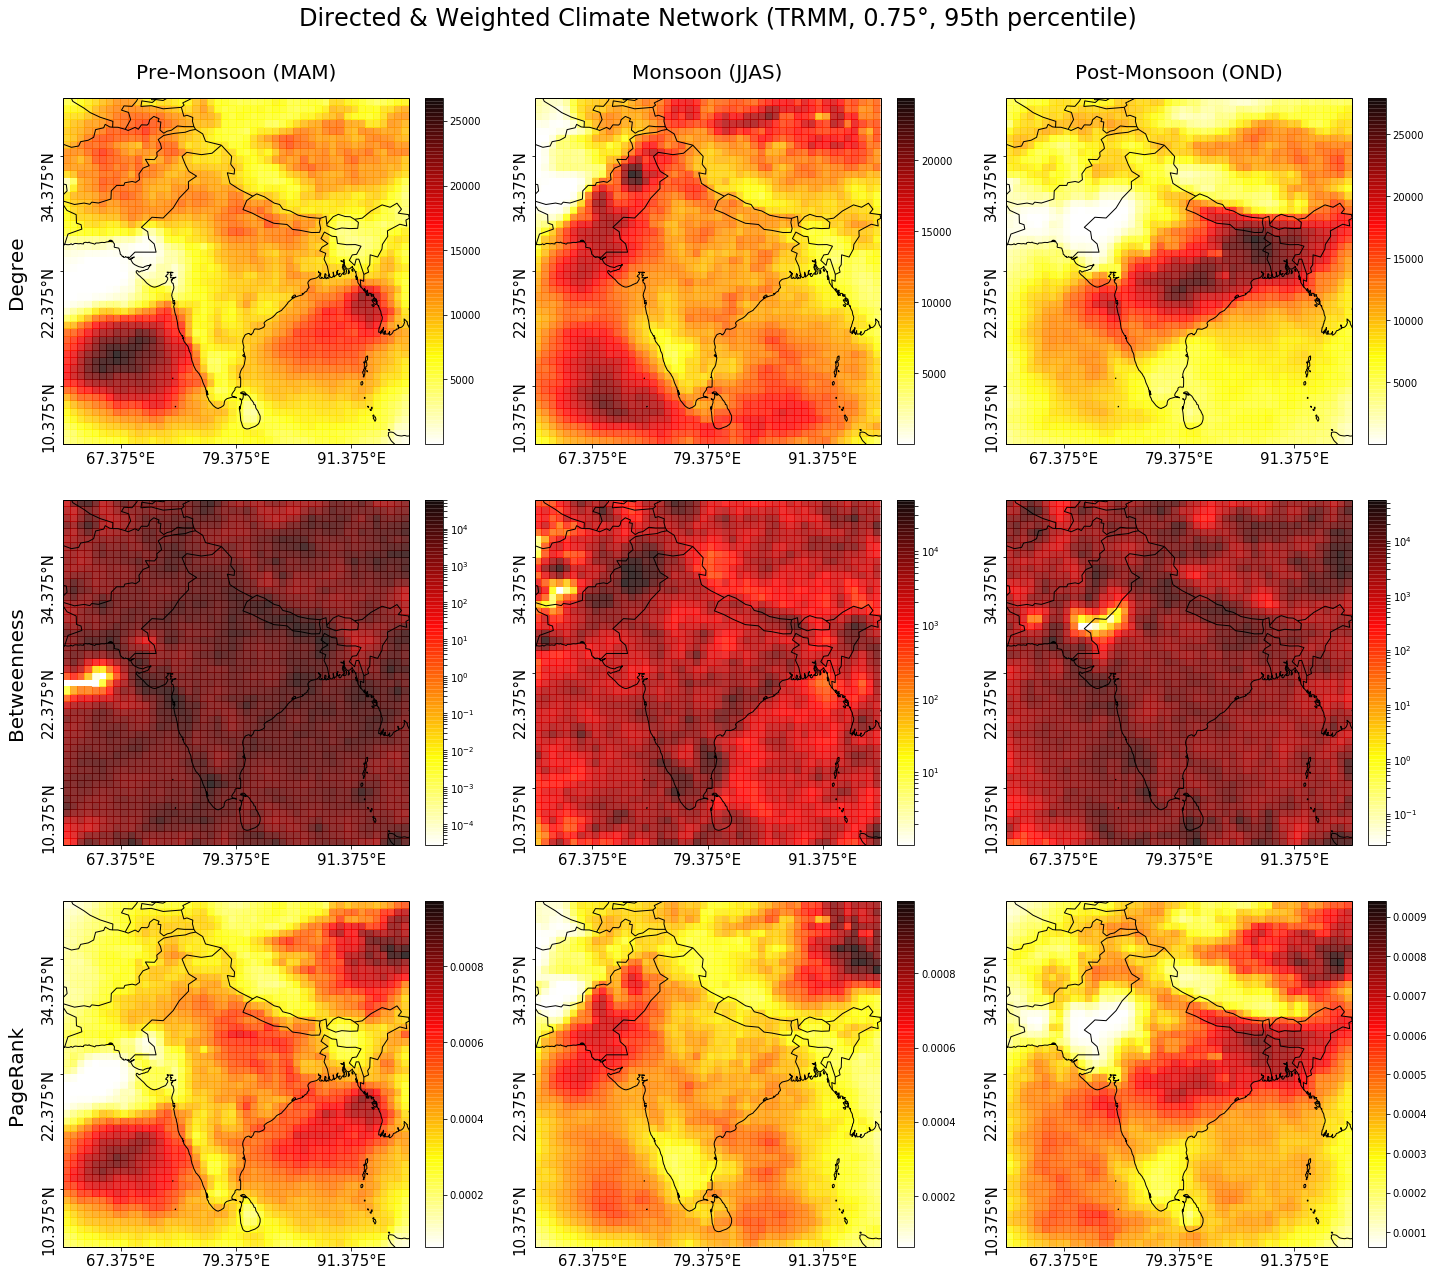
\includegraphics[width=\linewidth]{{./99_appendix/img/event_sync_0.75-0.9_directed_weighted}.png}
  \caption{Climate network analysis for weighted, directed climate networks (based on TRMM at {0.75\degree} resolution and a threshold set at the 95th percentile).}
  \label{apx:climate_network_both}
\end{figure}

\begin{figure}[h]
  \centering
  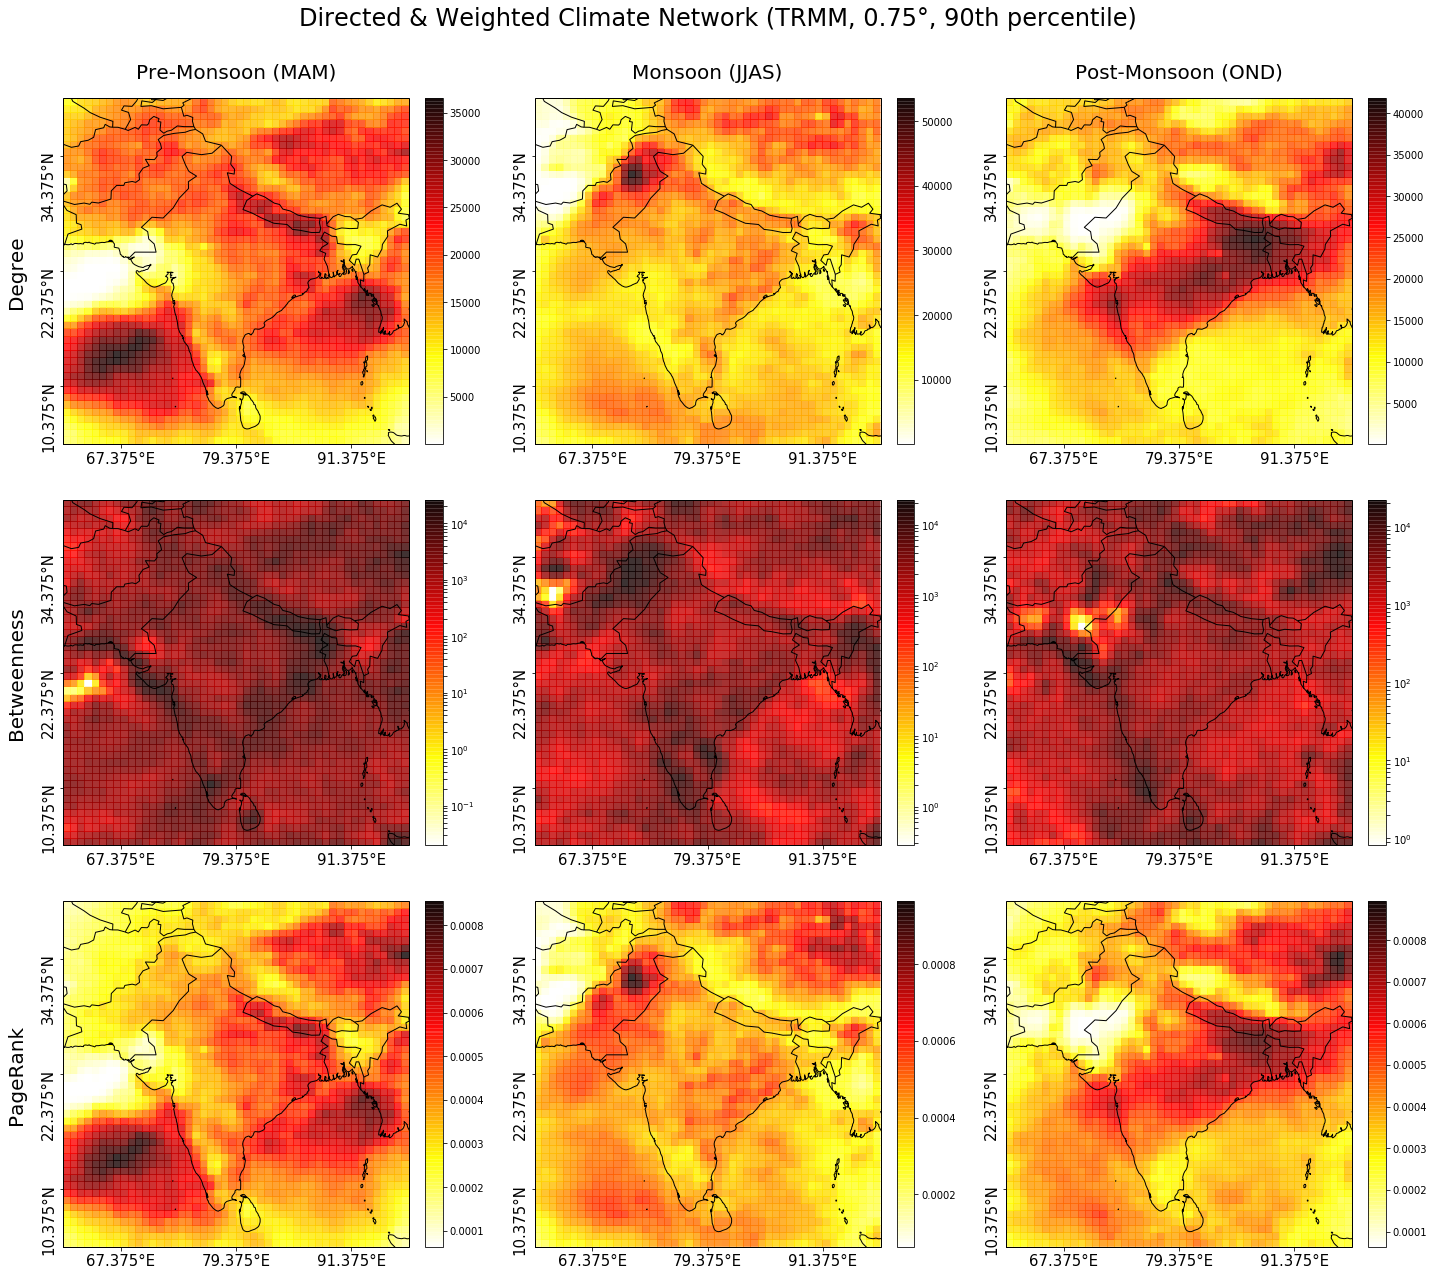
\includegraphics[width=\linewidth]{{./99_appendix/img/event_sync_0.75-0.9_directed_weighted_90}.png}
  \caption{Climate network analysis for weighted, directed climate networks (based on TRMM at {0.75\degree} resolution and a threshold set at the 90th percentile).}
  \label{apx:climate_network_both}
\end{figure}

\clearpage
\section{Neural Network Results}
\label{apx:nn_evaluation}

\begin{figure}[h]
  \centering
  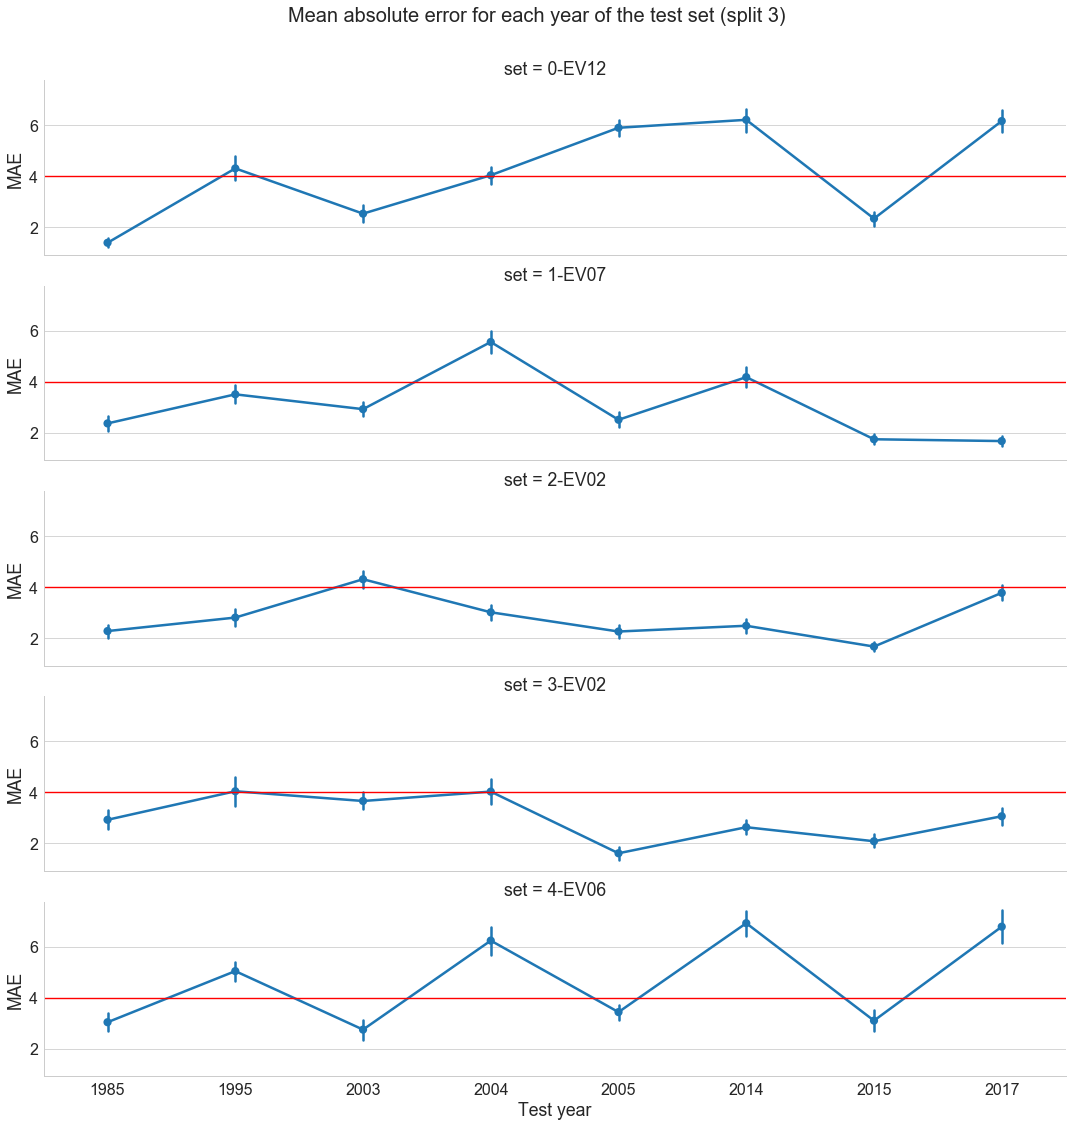
\includegraphics[width=\linewidth]{./99_appendix/img/prediction_years_ci.png}
  \caption{Yearly mean-absolute error (with 0.95 CI) averaged over the predictions of the final experiments on the test set (1985, 1995, 2003, 2004, 2005, 2014, 2015, 2017).}
  \label{apx:prediction_years_ci}
\end{figure}

\begin{figure}[h]
  \centering
  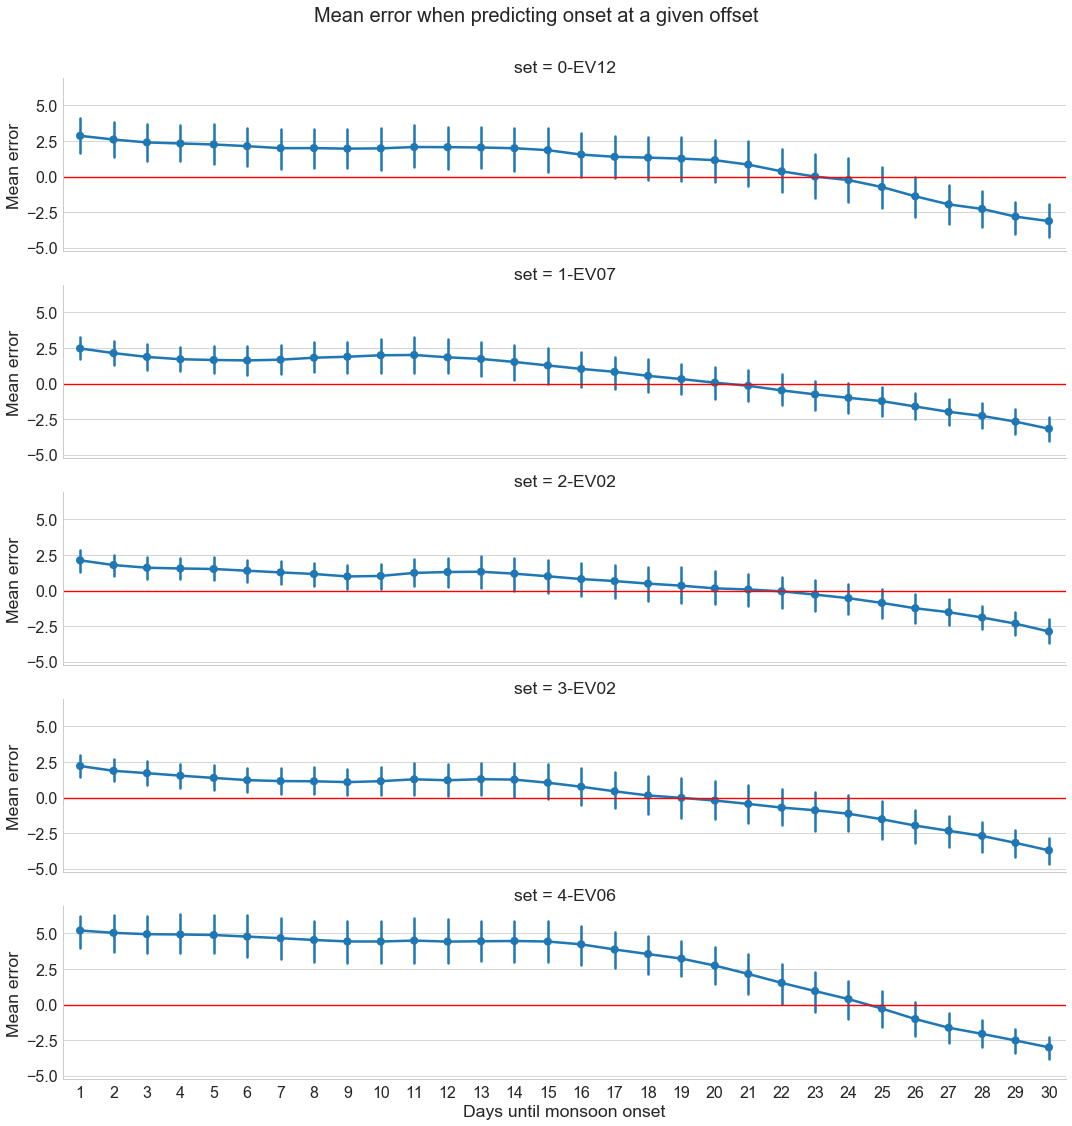
\includegraphics[width=\linewidth]{./99_appendix/img/prediction_error_offset_split.png}
  \caption{Mean error (with 0.95 CI) of each offset from MoK, averaged over the predictions of the final experiments on the test set (1985, 1995, 2003, 2004, 2005, 2014, 2015, 2017).}
  \label{apx:prediction_error_offset_ci}
\end{figure}

\begin{figure}[h]
  \centering
  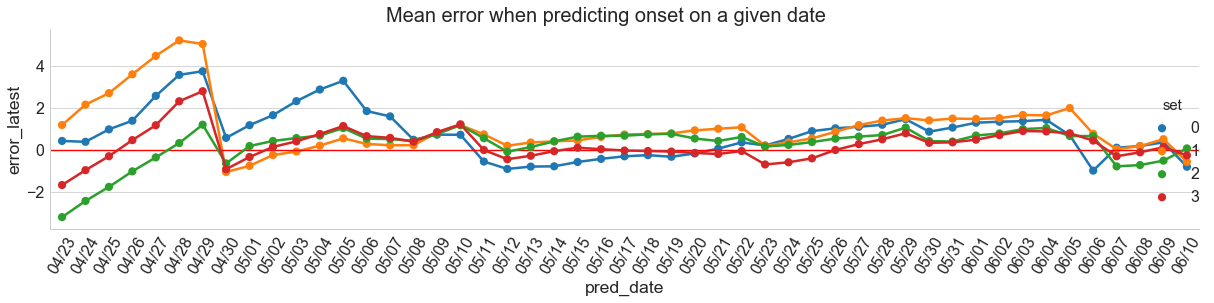
\includegraphics[width=\linewidth]{./99_appendix/img/prediction_error_dates.png}
  \caption{Mean error (with 0.95 CI) of each prediction date previous to MoK, averaged over the predictions of the final experiments on the test set (1985, 1995, 2003, 2004, 2005, 2014, 2015, 2017).}
  \label{apx:prediction_error_dates_ci}
\end{figure}

\begin{figure}[h]
  \centering
  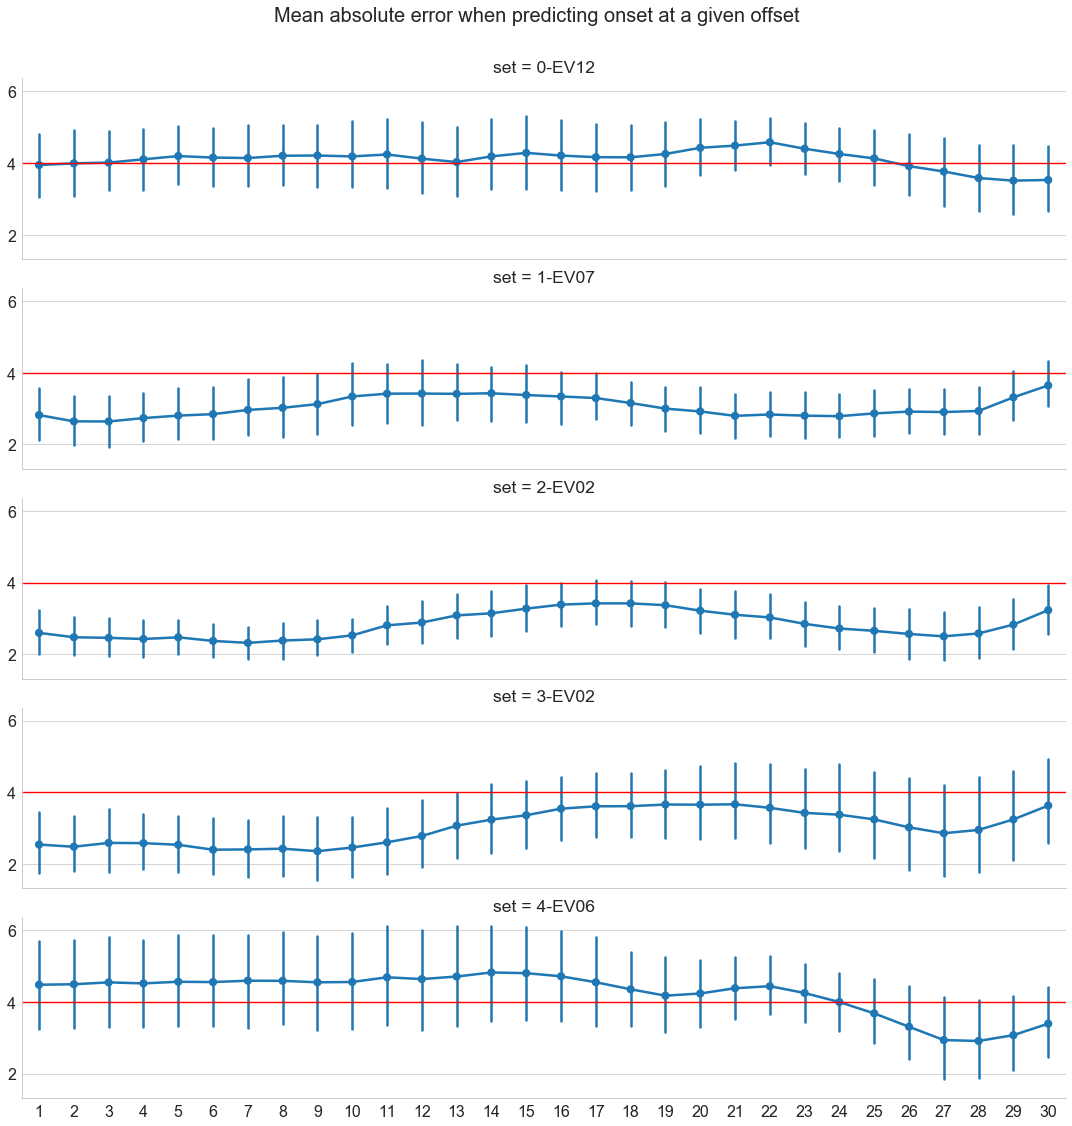
\includegraphics[width=\linewidth]{./99_appendix/img/prediction_accuracy_offset_split.png}
  \caption{Mean-absolute error (with 0.95 CI) of each offset from MoK, averaged over the predictions of the final experiments on the test set (1985, 1995, 2003, 2004, 2005, 2014, 2015, 2017).}
  \label{apx:prediction_accuracy_offset_ci}
\end{figure}

\begin{figure}[h]
  \centering
  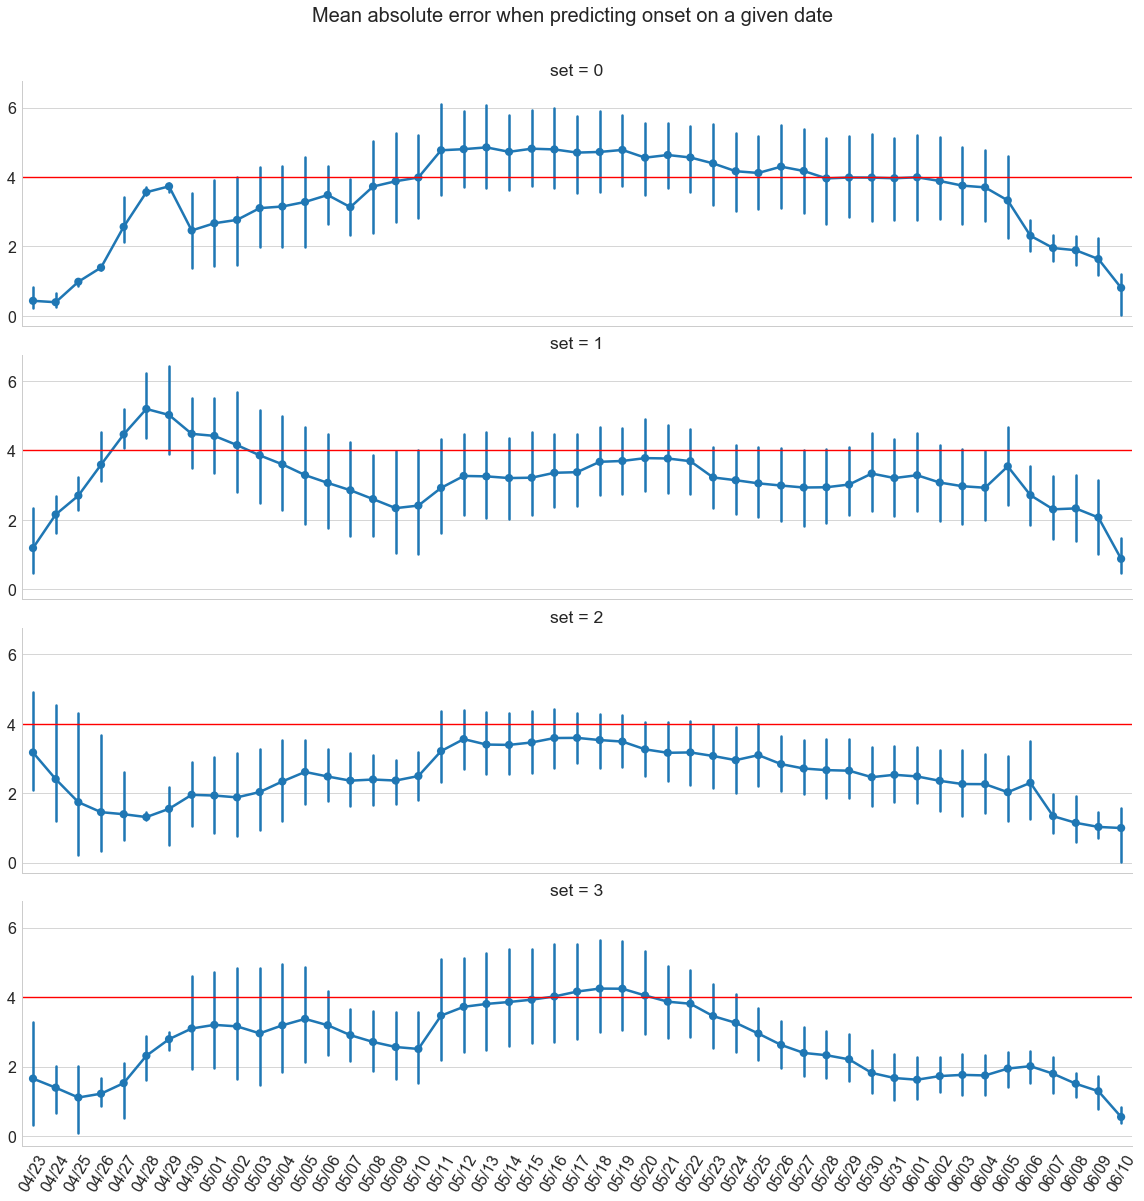
\includegraphics[width=\linewidth]{./99_appendix/img/prediction_accuracy_dates_split.png}
  \caption{Mean-absolute error (with 0.95 CI) of each prediction date previous to MoK, averaged over the predictions of the final experiments on the test set (1985, 1995, 2003, 2004, 2005, 2014, 2015, 2017).}
  \label{apx:prediction_accuracy_dates_ci}
\end{figure}
